\documentclass[10pt,twocolumn]{article}

% ---------------------------------------------------------------------
% Pacotes
% ---------------------------------------------------------------------
\usepackage[a4paper,top=2.1cm,bottom=2.3cm,left=1.7cm,right=1.7cm,columnsep=0.6cm]{geometry}
\usepackage[utf8]{inputenc}
\usepackage[T1]{fontenc}
\usepackage{times}
\usepackage{graphicx}
\usepackage{amsmath,amssymb}
\usepackage{booktabs}
\usepackage{array}
\usepackage{hyperref}
\usepackage{xcolor}
\usepackage{titlesec}
\usepackage{caption}
\usepackage{enumitem}
\usepackage{listings}
\usepackage{fancyhdr}

\hypersetup{colorlinks=true,linkcolor=blue,citecolor=blue,urlcolor=blue}

\titleformat{\section}{\large\bfseries}{\thesection}{0.5em}{}
\titleformat{\subsection}{\normalsize\bfseries}{\thesubsection}{0.5em}{}
\titlespacing*{\section}{0pt}{1.4ex plus 1ex minus .2ex}{0.8ex plus .2ex}
\titlespacing*{\subsection}{0pt}{1.1ex plus 1ex minus .2ex}{0.5ex plus .2ex}

\setlength{\parindent}{1em}
\captionsetup{font=small,labelfont=bf}

\lstset{
  basicstyle=\ttfamily\footnotesize,
  breaklines=true,
  columns=fullflexible,
  frame=single,
  numbers=left,
  numberstyle=\tiny,
  xleftmargin=1.2em,
  framexleftmargin=1.4em
}

\pagestyle{fancy}
\fancyhf{}
\renewcommand{\headrulewidth}{0pt}
\fancyfoot[C]{\thepage}

% ---------------------------------------------------------------------
% Cabecalho estilo "Journal" (similar ao template usado no TP.01)
% ---------------------------------------------------------------------
\newcommand{\journalheader}{%
  \begingroup
  \footnotesize\noindent
  Teoria dos Grafos e Computabilidade, 2025, Trabalho Pr\'atico N.02\par
  \rule{\linewidth}{0.4pt}\par
  This work is licensed under a Creative Commons Attribution 4.0 International License.
  \endgroup
}

\begin{document}

\makeatletter
\twocolumn[
  \begin{@twocolumnfalse}
    \journalheader
    \vspace{0.6em}
    \begin{center}
      {\LARGE\bfseries O Problema dos $k$-Centros: Algoritmo Exato via Busca Bin\'aria com Branch-and-Bound versus Heur\'istica de Aproxima\c{c}\~ao de Gonzalez\par}
      \vspace{0.9em}
      {\large
        Jo\~ao Comini Cesar de Andrade
        \quad
        Rafael Rehfeld Martins de Oliveira
        \par}
      \vspace{0.4em}
      {\small
        [ Pontif\'icia Universidade Cat\'olica de Minas Gerais | jccandrade@sga.pucminas.br ]\par
        [ Pontif\'icia Universidade Cat\'olica de Minas Gerais | rafael.oliveira.1508947@sga.pucminas.br ]
      \par}
      \vspace{0.2em}
      {\small Pontif\'icia Universidade Cat\'olica de Minas Gerais (PUC Minas), Brasil.\par}
    \end{center}
    \vspace{0.8em}

    \noindent\textbf{Resumo.} Este trabalho aborda o problema dos $k$-centros, uma tarefa
    cl\'assica de \emph{clustering} e localiza\c{c}\~ao de facilidades que consiste em
    escolher $k$ v\'ertices de um grafo de modo a minimizar a maior dist\^ancia entre
    qualquer v\'ertice e seu centro mais pr\'oximo. S\~ao implementadas e comparadas duas
    abordagens: um m\'etodo exato, baseado em busca bin\'aria sobre os valores de
    dist\^ancia combinada com um teste de viabilidade resolvido por
    \emph{branch-and-bound} sobre Cobertura de Conjuntos, e a heur\'istica de Gonzalez,
    uma $2$-aproxima\c{c}\~ao gulosa de \emph{farthest-point clustering}. Os m\'etodos
    foram avaliados nas 40 inst\^ancias de p-medianas da OR-Library (100 a 900 v\'ertices).
    Os resultados mostram que o m\'etodo exato s\'o \'e trat\'avel para inst\^ancias
    pequenas e, sobretudo, para valores baixos de $k$, tornando-se invi\'avel
    (\textgreater 5 minutos) j\'a a partir de inst\^ancias intermedi\'arias, enquanto a
    heur\'istica de Gonzalez resolve todas as inst\^ancias em milissegundos, com fator de
    aproxima\c{c}\~ao emp\'irico m\'edio de $1{,}50$ (ou seja, um erro m\'edio de
    aproximadamente $50\%$ acima do raio \'otimo), sempre dentro do limite te\'orico de
    $2{,}0$ ($100\%$ de erro).

    \vspace{0.6em}
    \noindent\textbf{Keywords:} Problema dos $k$-Centros, Algoritmos de Aproxima\c{c}\~ao,
    Heur\'istica de Gonzalez, Branch-and-Bound, Cobertura de Conjuntos, OR-Library.

    \vspace{1.0em}
  \end{@twocolumnfalse}
]
\makeatother

% =======================================================================
\section{Introdu\c{c}\~ao}
% =======================================================================

O problema dos $k$-centros \'e uma tarefa cl\'assica de an\'alise de dados, intimamente
relacionada a t\'ecnicas de \emph{clustering}. Dado um conjunto de pontos com dist\^ancias
definidas entre cada par e um inteiro positivo $k$, o objetivo \'e selecionar $k$ pontos
(chamados \emph{centros}) de forma a minimizar a maior dist\^ancia entre qualquer ponto do
conjunto e o centro mais pr\'oximo a ele. Essa dist\^ancia m\'axima \'e denominada
\emph{raio} da solu\c{c}\~ao.

Esse problema aparece naturalmente em cen\'arios de localiza\c{c}\~ao de facilidades --
por exemplo, decidir em quais de um conjunto de hospitais devem ser instalados centros de
tratamento especializados, de modo que nenhum hospital fique excessivamente distante do
centro mais pr\'oximo -- e tamb\'em em tarefas de categoriza\c{c}\~ao, como segmentar
consumidores, alunos ou usu\'arios de uma rede social em perfis homog\^eneos. \'E
sabido que a resolu\c{c}\~ao exata do problema \'e computacionalmente dif\'icil em
inst\^ancias grandes (o problema de decis\~ao associado \'e $\mathrm{NP}$-completo, por
redu\c{c}\~ao a Cobertura de Conjuntos), o que motiva o uso de algoritmos aproximados.

Neste trabalho, implementam-se e comparam-se duas abordagens distintas para o problema dos
$k$-centros:

\begin{enumerate}[leftmargin=1.3em,itemsep=1pt]
  \item \textbf{M\'etodo exato} (\texttt{KCentrosExato}): busca bin\'aria sobre os
  valores candidatos de raio, combinada com um teste de viabilidade \emph{exato},
  resolvido por enumera\c{c}\~ao exaustiva com poda (\emph{branch-and-bound}) sobre o
  problema de Cobertura de Conjuntos;
  \item \textbf{Heur\'istica aproximada} (\texttt{KCentrosGonzalez}): o algoritmo guloso
  de Gonzalez (\emph{farthest-point traversal}), que garante fator de aproxima\c{c}\~ao
  $2$ em rela\c{c}\~ao ao raio \'otimo.
\end{enumerate}

As duas implementa\c{c}\~oes s\~ao avaliadas sobre as 40 inst\^ancias de p-medianas da
OR-Library (\texttt{pmed1.txt} a \texttt{pmed40.txt}), com tamanhos de $100$ a $900$
v\'ertices, comparando-se efic\'acia (qualidade da solu\c{c}\~ao, medida pelo fator de
aproxima\c{c}\~ao em rela\c{c}\~ao ao raio \'otimo informado no enunciado) e efici\^encia
(tempo de execu\c{c}\~ao), \`a medida que o tamanho da inst\^ancia e o valor de $k$
aumentam.

% =======================================================================
\section{Referencial Te\'orico}
% =======================================================================

\subsection{Defini\c{c}\~ao Formal do Problema}

Dada uma cole\c{c}\~ao de pontos $V$ com dist\^ancias definidas para cada par pela
fun\c{c}\~ao $d : V \times V \mapsto \mathbb{R}^{+}$, o problema dos $k$-centros consiste
em encontrar um conjunto $C \subseteq V$, com $|C| \leq k$, de forma que a maior
dist\^ancia de um v\'ertice $v \in V$ ao centro mais pr\'oximo seja m\'inima, isto \'e,
minimizar
\[
  r(C) = \max_{v \in V} \min_{c \in C} d(v, c).
\]
Fixados os centros $C$, cada v\'ertice \'e implicitamente associado ao centro mais
pr\'oximo, definindo uma parti\c{c}\~ao de $V$ em at\'e $k$ \emph{clusters}.

\subsection{Equival\^encia com Cobertura de Conjuntos e Dificuldade}

Para um raio candidato $r$ fixo, perguntar se existe $C$, $|C|\leq k$, tal que todo
v\'ertice est\'a a dist\^ancia $\leq r$ de algum centro em $C$, \'e exatamente uma
inst\^ancia do problema de Cobertura de Conjuntos: cada v\'ertice $u$ define o
subconjunto $S_u = \{v \in V \mid d(u,v) \leq r\}$ de v\'ertices que ele consegue cobrir
caso seja escolhido como centro, e deseja-se saber se \'e poss\'ivel cobrir $V$ com
no m\'aximo $k$ desses subconjuntos \cite{garey1979}. Como Cobertura de Conjuntos \'e
$\mathrm{NP}$-completo, o problema de decis\~ao dos $k$-centros tamb\'em o \'e, e,
consequentemente, a vers\~ao de otimiza\c{c}\~ao \'e $\mathrm{NP}$-dif\'icil.

\subsection{Redu\c{c}\~ao da Otimiza\c{c}\~ao a uma Sequ\^encia de Decis\~oes}

Hochbaum e Shmoys mostram que o raio \'otimo $r^{*}$ pertence necessariamente ao
conjunto finito de dist\^ancias par a par $\{d(u,v) \mid u,v \in V\}$
\cite{hochbaum1985}. Isso permite reduzir o problema de otimiza\c{c}\~ao a uma busca
sobre esse conjunto ordenado de valores: para cada raio candidato, resolve-se o problema
de decis\~ao correspondente (vi\'avel ou n\~ao), e busca-se o menor raio vi\'avel --
naturalmente, por busca bin\'aria, j\'a que a viabilidade \'e mon\'otona em $r$ (se um
raio \'e vi\'avel, qualquer raio maior tamb\'em \'e).

\subsection{N\~ao-Aproximabilidade Abaixo de Fator 2}

Hochbaum e Shmoys tamb\'em demonstram que, a menos que $\mathrm{P}=\mathrm{NP}$, n\~ao
existe algoritmo de aproxima\c{c}\~ao para o problema dos $k$-centros com fator menor que
$2$ \cite{hochbaum1985}. Esse resultado situa a heur\'istica de Gonzalez, descrita a
seguir, como assintoticamente \'otima entre os algoritmos polinomiais conhecidos para o
problema.

\subsection{Heur\'istica de Gonzalez (Farthest-Point Clustering)}

Gonzalez propõe um algoritmo guloso que constr\'oi os $k$ centros iterativamente: o
primeiro centro \'e escolhido arbitrariamente e, a cada passo seguinte, escolhe-se como
novo centro o v\'ertice com a maior dist\^ancia m\'inima ao conjunto de centros j\'a
selecionado \cite{gonzalez1985}. Esse procedimento garante que o raio final obtido
\'e, no m\'aximo, o dobro do raio \'otimo $r^{*}$ -- a prova segue de um argumento de
pombos: se houvesse $k+1$ pontos mutuamente a dist\^ancia $> 2r^{*}$, pela
desigualdade triangular nenhum centro \'otimo poderia cobrir dois deles
simultaneamente com raio $r^{*}$, contradizendo a exist\^encia de uma solu\c{c}\~ao
\'otima com apenas $k$ centros.

\subsection{Floyd-Warshall}

Como as inst\^ancias da OR-Library fornecem um grafo esparso com pesos nas arestas (e
n\~ao diretamente a matriz de dist\^ancias completa exigida pela formula\c{c}\~ao do
problema), \'e necess\'ario pr\'e-processar as dist\^ancias de menor custo entre todos
os pares de v\'ertices. Isso \'e feito com o algoritmo de Floyd-Warshall, de
complexidade $O(n^3)$ \cite{cormen2009}.

% =======================================================================
\section{Metodologia}
% =======================================================================

\subsection{Inst\^ancias de Teste}

Conforme exigido pelo enunciado do trabalho, as implementa\c{c}\~oes foram testadas com
as 40 inst\^ancias do problema (n\~ao capacitado) das p-medianas da OR-Library
(\texttt{pmed1.txt} a \texttt{pmed40.txt}) \cite{beasley1990}. Embora o problema das
p-medianas use uma fun\c{c}\~ao objetivo diferente (soma das dist\^ancias, em vez do
m\'aximo), a mesma estrutura de grafo \'e reaproveitada como entrada para o problema dos
$k$-centros, conforme indicado no enunciado. Cada arquivo cont\'em, na primeira linha, o
n\'umero de v\'ertices $n$, o n\'umero de arestas $m$ e o n\'umero de centros $k$,
seguidos por $m$ linhas no formato \texttt{(u, v, peso)}. A Tabela~\ref{tab:instancias}
resume as caracter\'isticas das inst\^ancias e os valores de raio \'otimo fornecidos no
enunciado, usados como refer\^encia para o c\'alculo do fator de aproxima\c{c}\~ao.

\begin{table}[t]
\centering
\caption{Faixas de tamanho das 40 inst\^ancias utilizadas.}
\label{tab:instancias}
\small
\begin{tabular}{lccc}
\toprule
$|V|$ & Inst\^ancias & $k$ (faixa) & Raio \'otimo (faixa) \\
\midrule
100--900 & pmed1--pmed40 & 5--200 & 9--127 \\
\bottomrule
\end{tabular}
\end{table}

\subsection{Algoritmo Exato}

O m\'etodo exato realiza uma busca bin\'aria sobre os valores distintos de dist\^ancia
entre pares de v\'ertices (obtidos ap\'os Floyd-Warshall). Para cada raio candidato $r$,
testa-se a viabilidade resolvendo, de forma exaustiva, o problema de Cobertura de
Conjuntos correspondente: a cada passo, escolhe-se o v\'ertice ainda descoberto com
\textbf{menor n\'umero de candidatos capazes de cobri-lo} (heur\'istica
\emph{most-constrained-first}, usada apenas para reduzir o fator de ramifica\c{c}\~ao
m\'edio -- sem comprometer a corre\c{c}\~ao do resultado) e ramifica-se sobre cada um
desses candidatos, com poda quando o n\'umero de centros j\'a utilizados atinge $k$ sem
cobrir todos os v\'ertices. Por n\~ao empregar nenhuma heur\'istica na decis\~ao de
viabilidade em si, o m\'etodo \'e garantidamente exato, ao custo de complexidade
exponencial no pior caso.

\subsection{Heur\'istica de Gonzalez}

A heur\'istica mant\'em, para cada v\'ertice $v$, a dist\^ancia m\'inima
$\mathit{distMin}[v]$ at\'e o conjunto de centros escolhido at\'e o momento. O primeiro
centro \'e o v\'ertice de \'indice $0$; a cada itera\c{c}\~ao subsequente, escolhe-se o
v\'ertice que maximiza $\mathit{distMin}[v]$ como novo centro, e o vetor \'e atualizado em
$O(n)$. Ap\'os a escolha dos $k$ centros, o raio reportado \'e
$\max_v \mathit{distMin}[v]$.

\subsection{M\'etricas e Protocolo Experimental}

Para cada inst\^ancia e m\'etodo, foram registrados o \textbf{raio obtido}, o
\textbf{fator de aproxima\c{c}\~ao} ($\mathrm{FA} = \text{raio obtido} / \text{raio
\'otimo}$) e o \textbf{tempo de execu\c{c}\~ao} (em segundos). Como o m\'etodo exato
sempre encontra o raio \'otimo quando conclui, o $\mathrm{FA}$ s\'o \'e informativo para
a heur\'istica de Gonzalez; nesse caso, ele tamb\'em \'e expresso como um
\textbf{erro percentual} $\mathrm{Erro}(\%) = (\mathrm{FA}-1)\times 100\%$, isto \'e, o
quanto o raio aproximado excede o raio \'otimo (limite te\'orico de Gonzalez:
$\mathrm{FA}\leq 2 \Leftrightarrow \mathrm{Erro}\leq 100\%$).

A heur\'istica de Gonzalez \'e sempre executada, em todas as 40 inst\^ancias. J\'a o
m\'etodo exato \'e executado em uma \emph{thread} separada com um limite de tempo de
$300$ segundos (5 minutos); caso o limite seja excedido, a execu\c{c}\~ao \'e
interrompida e o resultado \'e descartado -- no \texttt{resultados.csv}, essas
inst\^ancias aparecem marcadas com \texttt{-1} nas colunas \texttt{exato\_raio},
\texttt{exato\_fa} e \texttt{exato\_tempo\_s}, indicando que o m\'etodo exato
\textbf{n\~ao conseguiu terminar dentro do limite de tempo} para aquela inst\^ancia, e
que, portanto, somente a heur\'istica de Gonzalez fornece uma solu\c{c}\~ao
(aproximada) nesses casos.

% =======================================================================
\section{Implementa\c{c}\~ao}
% =======================================================================

A implementa\c{c}\~ao foi realizada em Java, organizada em tr\^es classes principais:
\texttt{KCentrosExato.java}, \texttt{KCentrosGonzalez.java} e
\texttt{Experimentos.java}, al\'em das 40 inst\^ancias da OR-Library na pasta
\texttt{instancias/}.

\subsection{Leitura de Inst\^ancias e Pr\'e-processamento}

O m\'etodo \texttt{lerInstancia} (id\^entico nas duas classes de solu\c{c}\~ao) l\^e o
cabe\c{c}alho \texttt{(n, m, k)} e as $m$ arestas no formato da OR-Library, montando uma
matriz de adjac\^encia inicializada com $\infty$ (e $0$ na diagonal). Em seguida,
\texttt{floydWarshall} calcula a matriz de dist\^ancias de menor custo entre todos os
pares, em $O(n^3)$, necess\'aria pois a formula\c{c}\~ao do problema dos $k$-centros
pressup\~oe um grafo completo de dist\^ancias.

\subsection{KCentrosExato: Busca Bin\'aria + Branch-and-Bound}

O m\'etodo \texttt{resolve()} coleta os valores distintos de dist\^ancia, ordena-os e
realiza busca bin\'aria, chamando \texttt{verificaViabilidadeExata(r)} para cada raio
candidato. Essa fun\c{c}\~ao constr\'oi, para cada v\'ertice $v$, a lista de candidatos
que o cobrem com raio $r$, e delega a busca para \texttt{buscaExaustiva}, que implementa
o \emph{branch-and-bound} sobre Cobertura de Conjuntos descrito a seguir.

\begin{lstlisting}[caption={Esqueleto do branch-and-bound (most-constrained-first).},label={lst:bb}]
buscaExaustiva(coberto, centros, total):
  se total == n: retorna centros (solucao)
  se |centros| == k: retorna null (poda)
  v := vertice descoberto com menos
       candidatos que o cobrem
  para cada candidato de cobrePor[v]:
    aplica candidato (marca cobertos)
    resultado := buscaExaustiva(...)
    desfaz marcacao (backtracking)
    se resultado != null: retorna resultado
  retorna null
\end{lstlisting}

A escolha do v\'ertice mais restrito antes de ramificar (linhas 4--5) n\~ao altera a
corre\c{c}\~ao -- esse v\'ertice precisa ser coberto de qualquer forma -- mas reduz
substancialmente o fator de ramifica\c{c}\~ao m\'edio na pr\'atica, por podar cedo os
ramos inv\'iaveis.

\subsection{KCentrosGonzalez: Farthest-Point Greedy}

A implementa\c{c}\~ao segue diretamente o algoritmo de Gonzalez: um la\c{c}o de $k-1$
itera\c{c}\~oes que, a cada passo, varre o vetor $\mathit{distMin}$ em $O(n)$ para
encontrar o pr\'oximo centro e atualiz\'a-lo, resultando em complexidade total
$O(k \cdot n)$ ap\'os o pr\'e-processamento de Floyd-Warshall.

\subsection{Experimentos.java: Orquestra\c{c}\~ao}

A classe \texttt{Experimentos} percorre as 40 inst\^ancias, executa sempre a
heur\'istica de Gonzalez e, para o m\'etodo exato, inicia uma \texttt{Thread} dedicada e
aguarda sua conclus\~ao por at\'e \texttt{LIMITE\_MS = 300\_000} milissegundos
(\texttt{worker.join(LIMITE\_MS)}); se a \emph{thread} ainda estiver viva ap\'os esse
prazo, ela \'e interrompida e o resultado \'e descartado. Os raios \'otimos de
refer\^encia (Tabela 1 do enunciado) est\~ao embutidos no vetor \texttt{RAIOS\_OTIMOS} e
s\~ao usados apenas para calcular o fator de aproxima\c{c}\~ao de cada m\'etodo. Todos os
resultados s\~ao impressos em formato tabular e gravados em \texttt{resultados.csv}.

% =======================================================================
\section{Experimentos e Resultados}
% =======================================================================

Os experimentos foram executados sobre as 40 inst\^ancias \texttt{pmed1}--\texttt{pmed40}
($n$ entre 100 e 900, $k$ entre 5 e 200). A Tabela~\ref{tab:resultados} apresenta os
resultados completos: raio \'otimo de refer\^encia, raio e tempo obtidos pelo m\'etodo
exato (quando conclu\'ido dentro do limite de 300s) e pela heur\'istica de Gonzalez.

\begin{table*}[t]
\centering
\caption{Resultados completos para as 40 inst\^ancias (raio \'otimo conforme enunciado; ``--'' indica que o m\'etodo exato \textbf{n\~ao concluiu em 300s} -- nesses casos, o \texttt{resultados.csv} traz \texttt{-1}, e apenas a heur\'istica de Gonzalez resolve a inst\^ancia. Erro$_G$ = $(\mathrm{FA}_G-1)\times100\%$ \'e o quanto o raio de Gonzalez excede o raio \'otimo.).}
\label{tab:resultados}
\footnotesize
\begin{tabular}{rrrr|rrr|rrrr}
\toprule
Inst. & $n$ & $k$ & Raio \'ot. & Exato & FA$_E$ & $T_E$(s) & Gonzalez & FA$_G$ & Erro$_G$ & $T_G$(s) \\
\midrule
1  & 100 & 5   & 127 & 127 & 1,00 & 0,370   & 186 & 1,46 & 46,5\% & 0,002 \\
2  & 100 & 10  & 98  & 98  & 1,00 & 6,371   & 131 & 1,34 & 33,7\% & 0,000 \\
3  & 100 & 10  & 93  & 93  & 1,00 & 8,751   & 154 & 1,66 & 65,6\% & 0,000 \\
4  & 100 & 20  & 74  & 74  & 1,00 & 70,688  & 114 & 1,54 & 54,0\% & 0,000 \\
5  & 100 & 33  & 48  & 48  & 1,00 & 34,352  & 71  & 1,48 & 47,9\% & 0,001 \\
6  & 200 & 5   & 84  & 84  & 1,00 & 0,683   & 138 & 1,64 & 64,3\% & 0,000 \\
7  & 200 & 10  & 64  & --  & --   & --      & 96  & 1,50 & 50,0\% & 0,000 \\
8  & 200 & 20  & 55  & --  & --   & --      & 82  & 1,49 & 49,1\% & 0,000 \\
9  & 200 & 40  & 37  & --  & --   & --      & 57  & 1,54 & 54,0\% & 0,000 \\
10 & 200 & 67  & 20  & --  & --   & --      & 31  & 1,55 & 55,0\% & 0,001 \\
11 & 300 & 5   & 59  & 59  & 1,00 & 0,633   & 73  & 1,24 & 23,7\% & 0,000 \\
12 & 300 & 10  & 51  & 51  & 1,00 & 172,426 & 71  & 1,39 & 39,2\% & 0,001 \\
13 & 300 & 30  & 35  & --  & --   & --      & 59  & 1,69 & 68,6\% & 0,000 \\
14 & 300 & 60  & 26  & --  & --   & --      & 40  & 1,54 & 53,8\% & 0,003 \\
15 & 300 & 100 & 18  & --  & --   & --      & 25  & 1,39 & 38,9\% & 0,002 \\
16 & 400 & 5   & 47  & --  & --   & --      & 84  & 1,79 & 78,7\% & 0,001 \\
17 & 400 & 10  & 39  & --  & --   & --      & 56  & 1,44 & 43,6\% & 0,001 \\
18 & 400 & 40  & 28  & --  & --   & --      & 44  & 1,57 & 57,1\% & 0,000 \\
19 & 400 & 80  & 18  & --  & --   & --      & 28  & 1,56 & 55,6\% & 0,000 \\
20 & 400 & 133 & 13  & --  & --   & --      & 19  & 1,46 & 46,2\% & 0,000 \\
21 & 500 & 5   & 40  & --  & --   & --      & 53  & 1,32 & 32,5\% & 0,000 \\
22 & 500 & 10  & 38  & --  & --   & --      & 56  & 1,47 & 47,4\% & 0,000 \\
23 & 500 & 50  & 22  & --  & --   & --      & 34  & 1,55 & 54,6\% & 0,000 \\
24 & 500 & 100 & 15  & --  & --   & --      & 23  & 1,53 & 53,3\% & 0,000 \\
25 & 500 & 167 & 11  & --  & --   & --      & 15  & 1,36 & 36,4\% & 0,001 \\
26 & 600 & 5   & 38  & --  & --   & --      & 50  & 1,32 & 31,6\% & 0,000 \\
27 & 600 & 10  & 32  & --  & --   & --      & 43  & 1,34 & 34,4\% & 0,000 \\
28 & 600 & 60  & 18  & --  & --   & --      & 28  & 1,56 & 55,6\% & 0,000 \\
29 & 600 & 120 & 13  & --  & --   & --      & 19  & 1,46 & 46,2\% & 0,002 \\
30 & 600 & 200 & 9   & --  & --   & --      & 14  & 1,56 & 55,6\% & 0,001 \\
31 & 700 & 5   & 30  & --  & --   & --      & 42  & 1,40 & 40,0\% & 0,000 \\
32 & 700 & 10  & 29  & --  & --   & --      & 45  & 1,55 & 55,2\% & 0,000 \\
33 & 700 & 70  & 15  & --  & --   & --      & 25  & 1,67 & 66,7\% & 0,000 \\
34 & 700 & 140 & 11  & --  & --   & --      & 17  & 1,55 & 54,6\% & 0,003 \\
35 & 800 & 5   & 30  & --  & --   & --      & 38  & 1,27 & 26,7\% & 0,000 \\
36 & 800 & 10  & 27  & --  & --   & --      & 41  & 1,52 & 51,8\% & 0,000 \\
37 & 800 & 80  & 15  & --  & --   & --      & 25  & 1,67 & 66,7\% & 0,002 \\
38 & 900 & 5   & 29  & --  & --   & --      & 39  & 1,34 & 34,5\% & 0,000 \\
39 & 900 & 10  & 23  & --  & --   & --      & 35  & 1,52 & 52,2\% & 0,000 \\
40 & 900 & 90  & 13  & --  & --   & --      & 21  & 1,62 & 61,5\% & 0,002 \\
\bottomrule
\end{tabular}
\end{table*}

\subsection{Desempenho do M\'etodo Exato}

O m\'etodo exato concluiu dentro do limite de 300s em apenas 8 das 40 inst\^ancias:
pmed1--5 ($n=100$), pmed6 e pmed11 ($n=200$ e $n=300$, ambas com $k=5$) e pmed12
($n=300$, $k=10$). Em todos os casos conclu\'idos, o raio obtido coincide exatamente com
o raio \'otimo de refer\^encia ($\mathrm{FA}=1{,}00$), confirmando a corretude da
implementa\c{c}\~ao. A Figura~\ref{fig:tempo} ilustra, em escala logar\'itmica, o
crescimento abrupto do tempo do m\'etodo exato.

\'E not\'avel que o tempo de execu\c{c}\~ao do m\'etodo exato \emph{n\~ao} cresce de
forma monot\^onica apenas com $n$: a inst\^ancia pmed4 ($n=100$, $k=20$) levou
$70{,}7$s, mais do que pmed6 ($n=200$, $k=5$, apenas $0{,}68$s). O fator dominante \'e o
valor de $k$ -- quanto maior o n\'umero de centros a escolher, maior a profundidade da
\'arvore de busca do \emph{branch-and-bound} e maior o n\'umero de combina\c{c}\~oes
poss\'iveis de centros a explorar em cada teste de viabilidade. Esse efeito \'e ainda
mais evidente ao comparar pmed11 ($n=300$, $k=5$, $0{,}63$s) com pmed12 ($n=300$,
$k=10$, $172{,}4$s): dobrar $k$ de 5 para 10, mantendo $n$ fixo, multiplicou o tempo de
execu\c{c}\~ao por mais de 270 vezes. J\'a para $k \geq 30$ (pmed13 em diante) ou para
$k=10$ com $n \geq 400$ (pmed17), o m\'etodo exato n\~ao concluiu dentro do limite de 5
minutos em nenhum dos testes restantes, evidenciando a complexidade exponencial no pior
caso do teste de viabilidade.

\begin{figure}[t]
  \centering
  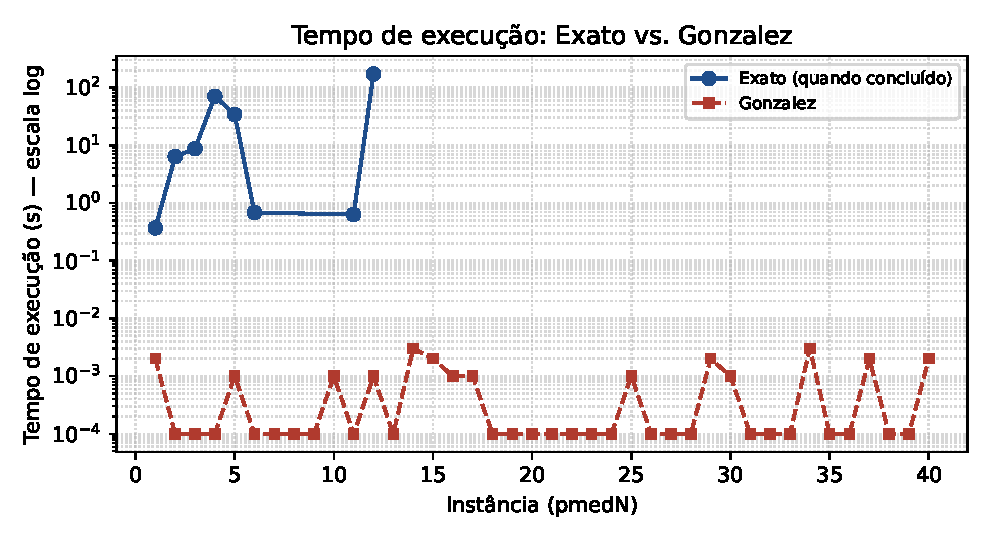
\includegraphics[width=\linewidth]{figs/tempo_comparativo.pdf}
  \caption{Tempo de execu\c{c}\~ao (escala log) do m\'etodo exato (apenas inst\^ancias
  conclu\'idas) e da heur\'istica de Gonzalez, por inst\^ancia.}
  \label{fig:tempo}
\end{figure}

\subsection{Desempenho da Heur\'istica de Gonzalez}

Em contraste direto, a heur\'istica de Gonzalez resolveu todas as 40 inst\^ancias --
incluindo a maior, com 900 v\'ertices -- em no m\'aximo 3 milissegundos, refletindo sua
complexidade polinomial $O(k \cdot n)$ ap\'os o pr\'e-processamento. O fator de
aproxima\c{c}\~ao variou entre $1{,}24$ (pmed11) e $1{,}79$ (pmed16), com m\'edia
emp\'irica de $1{,}50$ e desvio padr\~ao de $0{,}12$ -- portanto, sempre confortavelmente
abaixo do limite te\'orico de $2{,}0$ garantido por Gonzalez \cite{gonzalez1985}, como
mostra a Figura~\ref{fig:fa}. Em termos de erro percentual em rela\c{c}\~ao ao raio
\'otimo (coluna Erro$_G$ da Tabela~\ref{tab:resultados}), isso significa que a
heur\'istica errou, em m\'edia, $49{,}6\%$ acima do \'otimo, com m\'inimo de $23{,}7\%$
(pmed11) e m\'aximo de $78{,}7\%$ (pmed16) -- sempre dentro do limite te\'orico de
$100\%$ de erro ($\mathrm{FA}=2$). N\~ao h\'a tend\^encia clara de piora do fator de
aproxima\c{c}\~ao (ou do erro percentual) com o crescimento de $n$ ou $k$ nas
inst\^ancias testadas, sugerindo que o comportamento m\'edio da heur\'istica \'e
consideravelmente melhor do que sua garantia de pior caso para estas inst\^ancias da
OR-Library.

\begin{figure}[t]
  \centering
  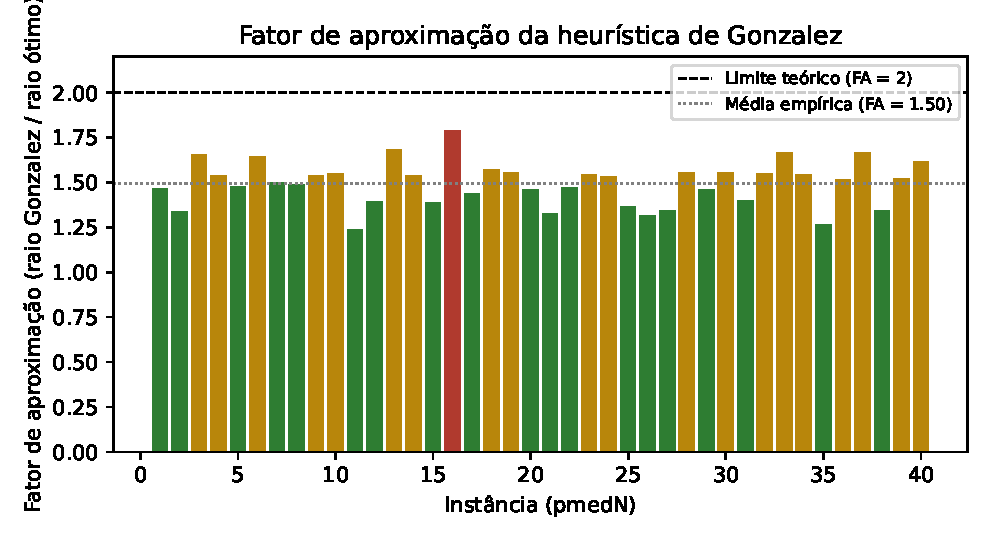
\includegraphics[width=\linewidth]{figs/fa_gonzalez.pdf}
  \caption{Fator de aproxima\c{c}\~ao da heur\'istica de Gonzalez em cada uma das 40
  inst\^ancias, com a m\'edia emp\'irica e o limite te\'orico de $2{,}0$.}
  \label{fig:fa}
\end{figure}

\subsection{An\'alise Comparativa}

Os resultados evidenciam o compromisso cl\'assico entre exatid\~ao e escalabilidade. O
m\'etodo exato garante a solu\c{c}\~ao \'otima ($\mathrm{FA}=1$), mas seu custo
exponencial restringe sua aplicabilidade pr\'atica a inst\^ancias pequenas e,
principalmente, a valores baixos de $k$ -- mesmo inst\^ancias com $n$ moderado (300
v\'ertices) tornam-se intrat\'aveis quando $k$ cresce. Esse comportamento \'e consistente
com a natureza do teste de viabilidade: o n\'umero de subconjuntos de centros de tamanho
$k$ a considerar cresce combinatorialmente com $k$, e a busca bin\'aria sobre o raio
multiplica esse custo por $O(\log n^2)$ testes de viabilidade.

Por outro lado, a heur\'istica de Gonzalez escala perfeitamente para todas as
inst\^ancias testadas, sacrificando otimalidade por uma garantia de qualidade
constante (fator $2$) que, na pr\'atica, se mostrou bem mais apertada ($\approx 1{,}5$
em m\'edia). Para aplica\c{c}\~oes reais envolvendo grafos de m\'edio a grande porte ou
valores de $k$ moderados a altos, a heur\'istica de Gonzalez \'e claramente a escolha
mais vi\'avel; o m\'etodo exato permanece \'util como refer\^encia de qualidade (\emph{
ground truth}) para validar heur\'isticas em inst\^ancias pequenas.

% =======================================================================
\section{Conclus\~ao}
% =======================================================================

Este trabalho implementou e comparou duas abordagens para o problema dos $k$-centros: um
m\'etodo exato baseado em busca bin\'aria com teste de viabilidade por
\emph{branch-and-bound} sobre Cobertura de Conjuntos, e a heur\'istica gulosa de
Gonzalez, com garantia te\'orica de $2$-aproxima\c{c}\~ao. Os experimentos sobre as 40
inst\^ancias de p-medianas da OR-Library confirmam que o m\'etodo exato, apesar de
garantir a solu\c{c}\~ao \'otima, \'e invi\'avel na pr\'atica assim que $k$ ultrapassa
valores pequenos (em torno de 10), independentemente do tamanho $n$ da inst\^ancia, em
raz\~ao da complexidade exponencial do teste de viabilidade subjacente. J\'a a
heur\'istica de Gonzalez resolveu todas as inst\^ancias -- inclusive a de 900 v\'ertices
-- em tempo desprez\'ivel, com fator de aproxima\c{c}\~ao emp\'irico m\'edio de
$1{,}50$ (erro m\'edio de $49{,}6\%$ acima do raio \'otimo), sempre respeitando o limite
te\'orico de $2{,}0$ ($100\%$ de erro). Conclui-se que, para
aplica\c{c}\~oes pr\'aticas em larga escala, a heur\'istica de Gonzalez \'e a op\c{c}\~ao
recomendada, reservando-se o m\'etodo exato para valida\c{c}\~ao em inst\^ancias
pequenas ou com poucos centros.

\section*{Disponibilidade de dados e materiais}
O c\'odigo-fonte com todas as implementa\c{c}\~oes (\texttt{KCentrosExato.java},
\texttt{KCentrosGonzalez.java}, \texttt{Experimentos.java}), as inst\^ancias utilizadas
e os resultados brutos (\texttt{resultados.csv}) acompanham a entrega deste trabalho.

% =======================================================================
\begin{thebibliography}{9}

\bibitem{beasley1990}
Beasley, J. E. (1990). OR-Library: Distributing test problems by electronic mail.
\textit{Journal of the Operational Research Society}, 41(11), 1069--1072.
DOI: \url{https://doi.org/10.1057/jors.1990.166}

\bibitem{cormen2009}
Cormen, T. H., Leiserson, C. E., Rivest, R. L., and Stein, C. (2009).
\textit{Introduction to Algorithms}. The MIT Press, third edition.

\bibitem{garey1979}
Garey, M. R., and Johnson, D. S. (1979). \textit{Computers and Intractability: A Guide
to the Theory of NP-Completeness}. W. H. Freeman and Company.

\bibitem{gonzalez1985}
Gonzalez, T. F. (1985). Clustering to minimize the maximum intercluster distance.
\textit{Theoretical Computer Science}, 38, 293--306.
DOI: \url{https://doi.org/10.1016/0304-3975(85)90224-5}

\bibitem{hochbaum1985}
Hochbaum, D. S., and Shmoys, D. B. (1985). A best possible heuristic for the $k$-center
problem. \textit{Mathematics of Operations Research}, 10(2), 180--184.
DOI: \url{https://doi.org/10.1287/moor.10.2.180}

\end{thebibliography}

\end{document}
